\documentclass[11pt,a4paper]{article}
\usepackage[utf8]{inputenc}
\usepackage[T1]{fontenc}
\usepackage[romanian]{babel}
\usepackage[margin=2cm]{geometry}
\usepackage{array}
\usepackage{tabularx}
\usepackage{enumitem}
\usepackage{graphicx}
\usepackage{setspace}
\usepackage{xcolor}
\usepackage{hyperref}
\usepackage{amssymb}
\setlength{\parindent}{0pt}
\newcommand{\fillline}[1][6cm]{\underline{\hspace{#1}}}
\newcommand{\fillbox}[1][0.4cm]{\framebox[#1]{\rule{0pt}{#1}}}
\newcommand{\checkboxempty}{$\square$}

\begin{document}

\noindent
\begin{minipage}[t]{0.40\textwidth}
\vspace{0pt}
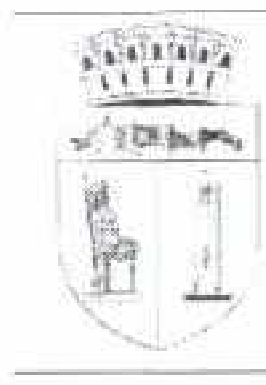
\includegraphics[height=1.5cm]{assets/stema-cluj.png}%
\hspace{0.2cm}%
\raisebox{0.5cm}{\parbox[t]{3.5cm}{\textbf{PRIMĂRIA}\\\textbf{CLUJ-NAPOCA}}}
\end{minipage}%
\begin{minipage}[t]{0.30\textwidth}
\centering
\vspace{0.4cm}

\includegraphics[width=3.5cm,height=0.9cm]{assets/barcode-801001.png}
\end{minipage}%
\begin{minipage}[t]{0.30\textwidth}
\raggedleft
\vspace{0.6cm}
Nr. \fillline[3cm] / \fillline[1cm]
\end{minipage}

\vspace{0.3cm}
\hrule
\vspace{0.5cm}

\begin{center}
\textbf{CERERE ŞI DECLARAŢIE PE PROPRIA RĂSPUNDERE}\\[0.3cm]
\textbf{A. CERERE}
\end{center}

\vspace{0.5cm}

\hspace{1cm}Subsemnatul/a \underline{ {{nume_complet}} }, CNP \underline{ {{cnp}} }, cu domiciliul/reședința în Cluj-Napoca, str. \underline{ {{strada}} } nr. \underline{ {{numar}} } ap. \underline{ {{apartament}} }, Telefon \underline{ {{telefon}} }, în calitate de persoană singură/reprezentant al unei familii în care există cel puțin o persoană aflată în una dintre următoarele situaţii (se bifează cu "x" caseta corespunzătoare):

\vspace{0.4cm}

\hspace{0.5cm}\checkboxempty\ persoane cu handicap grav sau accentuat, neinstituționalizate;

\vspace{0.2cm}

\hspace{0.5cm}\checkboxempty\ pensionari, invalizi, veterani, văduve de război, persoane deportate, prizonieri, persecutați politic, eroi martiri ai revoluției, orfani, ale căror venituri nete lunare pentru persoana singură sunt de până la 2600 lei și de până la 1700 lei/membru de familie;

\vspace{0.2cm}

\hspace{0.5cm}\checkboxempty\ șomeri înregistrați (cu/fără indemnizație de șomaj) ale căror venituri nete lunare pentru persoana singură sunt de până la 2600 lei și de până la 1700 lei/membru de familie;

\vspace{0.2cm}

\hspace{0.5cm}\checkboxempty\ beneficiari de venit minim de incluziune;

\vspace{0.2cm}

\hspace{0.5cm}\checkboxempty\ victimă a traficului de persoane;

\vspace{0.2cm}

\hspace{0.5cm}\checkboxempty\ victimă a violenței domestice.

\vspace{0.4cm}

\hspace{1cm}\textbf{Vă rog să-mi aprobaţi acordarea tichetelor sociale pe suport electronic în cadrul Programului social „Alimente".}

\vspace{0.3cm}

\hspace{1cm}\textbf{Declar pe propria răspundere} că nu am obligaţii de plată faţă de bugetul local.

\vspace{0.3cm}

\hspace{1cm}Menționez că am fost informat/ă cu privire la Regulamentul (UE) nr. 679/2016 al Parlamentului European şi al Consiliului Uniunii Europene privind protecţia persoanelor fizice în ceea ce priveşte prelucrarea datelor cu caracter personal şi privind libera circulaţie a acestor date \textit{şi de abrogare a Directivei 95/46/CE (Regulamentul general privind protecţia datelor) pus în aplicare prin Legea nr.190/2018}.

\vspace{0.3cm}

\hspace{1cm}\textbf{Declar că îmi dau consimțământul în mod expres} în ceea ce priveşte prelucrarea datelor mele cu caracter personal, precum şi în furnizarea datelor personale pentru a fi prelucrate, utilizate cu scopul acordării tichetelor sociale în cadrul Programului social ``Alimente''.

\vspace{0.3cm}

\hspace{1cm}Am înțeles această declarație de consimțământ și sunt de acord cu procesarea datelor mele cu caracter personal prin canalele de mai sus, în scopurile descrise în prezenta.

\vspace{0.4cm}

Anexez următoarele documente doveditoare:

\vspace{0.2cm}

\begin{enumerate}[leftmargin=2cm]
\item \underline{ {{document_1}} }
\item \underline{ {{document_2}} }
\item \underline{ {{document_3}} }
\item \fillline[12cm]
\item \fillline[12cm]
\item \fillline[12cm]
\item \fillline[12cm]
\item \fillline[12cm]
\end{enumerate}

\vspace{0.6cm}

\hspace{1cm}Data: \fillline[4cm] \hfill Semnătura, \fillline[5cm]\hspace{1cm}

\hfill (faţă)

\vspace{0.4cm}

\textbf{Atenție! Completați și Declarația de pe verso (întoarceți pagina)!}

\vfill
\hrule
\vspace{0.3cm}

\begin{minipage}[t]{0.65\textwidth}
www.primariaclujnapoca.ro\\
telefon: 0264/596.030\\
Cluj-Napoca, str. Moţilor, nr. 3
\end{minipage}%
\begin{minipage}[t]{0.35\textwidth}
\raggedleft

\includegraphics[width=3cm,height=0.7cm]{assets/barcode-801001.png}
\end{minipage}

\vspace{0.3cm}
\hrule
\vspace{0.2cm}

{\footnotesize
\textbf{Timp estimativ de completare: 10 minute}
}

\end{document}
